%%%%%%%%%%%%%%%%%%%%%%%%%%%%%%%%%%%%%%%%%%%%%%%%%%%%%%%%%%%%%%%%%%%%%%

% From jcapexample.tex
\RequirePackage[displaymath]{lineno}
\documentclass[a4paper,11pt]{article}
\pdfoutput=1 

% JCAP style
\usepackage{jcappub}
\usepackage[T1]{fontenc} % if needed
%\usepackage{lineno}

\usepackage{cancel}

% Stuff not in jcappub
\usepackage{aas_macros}
%\usepackage{xcolor}
\usepackage{tablefootnote}
\usepackage[displaymath]{lineno}
\usepackage{subfigure}
\usepackage{multirow}
\usepackage{amsmath}
\usepackage{cleveref}

%% Language and font encodings
%\usepackage[english]{babel}
%\usepackage[utf8x]{inputenc}
%\usepackage[T1]{fontenc}

\usepackage{enumitem}
\newcommand{\subscript}[2]{$#1 _ #2$}
%% Sets page size and margins
%\usepackage[a4paper,top=3cm,bottom=2cm,left=3cm,right=3cm,marginparwidth=1.75cm]{geometry}

%% Useful packages
%\usepackage{amsmath}
\usepackage{graphicx}
\usepackage[colorinlistoftodos]{todonotes}
%\usepackage[colorlinks=true, allcolors=blue]{hyperref}

%\usepackage{footmisc}
%\renewcommand\footnotelayout{\fontsize{10}{12}\selectfont}

\notoc


% Latex macros
%\input{fermiStyle.tex}




%%%%%%%%%%%%%%%%%%%%%%%%%%%%%%%%%%%%%%%%%%%%%%%%%%%%%%%%%%%%%%%%%%%%%%%%

\def\ie{{\it i.e.}}
\def\lsim{\:\raisebox{-0.5ex}{$\stackrel{\textstyle<}{\sim}$}\:}
\def\gsim{\:\raisebox{-0.5ex}{$\stackrel{\textstyle>}{\sim}$}\:}
\def\half{\textstyle{1\over2}}
\def\fouth{\textstyle{1\over4}}
\def\eighth{\textstyle{1\over8}}
\def\third{{\textstyle{1 \over 3}}}
\topmargin 1cm

\newcommand{\GEV}{\ensuremath{\,\textnormal{GeV}}}
\newcommand{\TEV}{\ensuremath{\,\textnormal{TeV}}}
\newcommand{\MEV}{\ensuremath{\,\textnormal{MeV}}}
\newcommand{\KEV}{\ensuremath{\,\textnormal{KeV}}}
\newcommand{\SEC}{\ensuremath{\,\textnormal{s}}}
\newcommand{\dropbox}{/Users/nicoviaux/Dropbox/} %Cambiar esta linea para editar
\newcommand{\folder}{Gravitino_Bounds/Paper/}
%\newcommand{\folder}{/media}

\newcommand*{\blue}{\textcolor{blue}}
\newcommand*{\red}{\textcolor{red}}

\interfootnotelinepenalty=10000


\begin{document}

\title{Gravitino dark matter with trilinear couplings to explain the anomalous positron fraction}

% Author list
\author[a,b]{Johannes~Buchner,}
\author[d]{Edson~Carquin,}
\author[c]{Marco~A.~D\'\i az,}
\author[a]{Germ\'an~A.~G\'omez-Vargas,\footnote{Now Corporate Data Scientist at \href{https://www.derco.cl/}{Derco},}}
\author[a]{Boris~Panes,}
\author[d]{Nicol\'as Viaux}

\affiliation[a]{Instituto de Astrof\'isica, Pontificia Universidad Cat\'olica de Chile, Avenida Vicu\~na Mackenna 4860, Santiago, Chile}
\affiliation[b]{Millenium Institute of Astrophysics, Vicu\~na MacKenna 4860, 7820436 Macul, Santiago, Chile}
\affiliation[c]{Instituto de F\'isica, Pontificia Universidad Cat\'olica de Chile, Avenida Vicu\~na Mackenna 4860, Santiago, Chile}
\affiliation[d]{Departamento de F\'isica y Centro Cient\'ifico- Tecnol\'ogico de Valpara\'iso (CCTVal), Universidad T\'ecnica Federico Santa Mar\'ia, Av. Espa\~na 1680, Valpara\'iso, Chile}

\emailAdd{johannes.buchner.acad@gmx.com} % orcid: 0000-0003-0426-6634
\emailAdd{edson.carquin@usm.cl}
\emailAdd{mad@susy.fis.puc.cl}
\emailAdd{ggomezv@uc.cl}
\emailAdd{bpanes@astro.puc.cl}
\emailAdd{nicolas.viaux@usm.cl}


%\pacs{95.35.+d,95.30.Cq,98.35.Gi}

\abstract{The flux of charged leptons measured by the space-based detectors PAMELA, AMS-02, CALET, DAMPE and Fermi-LAT presents anomalous behavior, \blue{in comparison to expectations from standard astrophysical sources}, as energy increase. In particular, AMS-02 observations provide compelling evidence for a new source of positrons and electrons. Its origin is still unknown, but successful scenarios include the contribution of dark matter and unresolved astrophysical sources, such as nearby pulsars. It has been shown that explanations based mostly on dark matter emission tend to overproduce gamma-rays, entering in conflict with measurements of the extra-galactic gamma-ray background (EGB). Although this situation seems to be quite generic, it ultimately depends on the particular properties of dark matter candidates. For instance, in this work we revisit a model that contains a gravitino as dark matter candidate, which is able to decay to standard model particles through trilinear R-parity violating couplings. \blue{Compared to the bilinear scenario, our model produces more electrons and positrons and fewer photons. When considering AMS-02 data alone, this model is compatible with EGB constraints. However, when DAMPE or CALET measurements of the sum of electrons and positrons are considered without the AMS-02 data, tensions appear. Therefore, to evaluate this model further, discrepancies between the data collected by these experiments need to be clarified.}}

%This model is able to produce more electrons and positrons and lesser photons, when compared to the bilinear scenario, which ultimately helps to reduce the mentioned conflicts with the EGB. Interestingly, when we consider only AMS-02 data, this model turn out to be compatible with the bounds from the EGB. However, when the sum of electrons and positrons measured by DAMPE or CALET are considered, instead of the analogous AMS-02 data, the tensions are back again. This implies that in order to determine the fate of this model, it becomes necessary to firstly clarify some discrepancies between the data collected by these experiments.} 

%\mathbf{on cosmic rays, }

\keywords{dark matter experiments, cosmic ray experiments, gamma ray experiments, dark matter theory}

\maketitle
%\flushbottom


\newpage
%%%%%%%%%%%%%%%%%%%%%%%%%%%%%%%%%%%%%%%%%%%%%%%%%%%%%%%%%%%%%%%%%%%%
\section{Introduction}
%%%%%%%%%%%%%%%%%%%%%%%%%%%%%%%%%%%%%%%%%%%%%%%%%%%%%%%%%%%%%%%%%%

The continuous and systematic analysis of the data collected by cosmic-ray detectors is one of the most direct ways to check and test the predictions of particle physics models that contain a candidate for dark matter (DM) which can annihilate or decay to Standard Model (SM) particles. \blue{For a review focused on the gravitino dark matter scenario we refer to~\cite{Grefe:2011dp} and~\cite{Hooper:2018kfv} for an updated and more general discussion.} 

Furthermore, this discussion becomes specially relevant since \blue{contemporary experiments present persistent and striking anomalies in cosmic-rays detection}. For instance, the energy spectrum of electrons and positrons measured by experiments such as PAMELA~\cite{Adriani:2008zr}, AMS-02~\cite{Accardo:2014lma,Aguilar:2014mma,Aguilar:2014fea}, CALET~\cite{Adriani:2018ktz}, DAMPE~\cite{Ambrosi:2017wek} and Fermi-LAT~\cite{Ackermann:2014usa} show noticeable discrepancies when compared to predictions based on standard astrophysical sources, such as cosmic-ray interactions or emissions from pulsars. Therefore, these experimental signals strongly suggest that extra sources of (primary) positrons are required in order to make sense of the data. 

In particular, it has been shown that the positron anomaly, reported by experiments such as PAMELA~\cite{Adriani:2008zr} and AMS-02~\cite{Accardo:2014lma}, can be well explained by considering a population of DM in agreement with standard density profiles, such as NFW, that can annihiliate or decay to charged leptons both as primary or secondary particles. This picture, however, seems to be in conflict with the measurementes of the extra galactic gamma-ray background (EGB) derived from Fermi-LAT and other gammar-ray detectors \cite{Grefe:2008zz,2012PhRvD..86h3506C,Ando:2015qda,Laletin:2016egv,Liu:2016ngs,Belotsky:2016tja}. Some of these explanations include modifications of (standard) DM density distributions. In general, it may be argued that a more realistic explanation of the anomalous data must include DM particles, probably with improved properties in comparison to current models, \blue{in addition to proper modelling} of astrophysical sources~\red{Refs from HAWC experiment and Hooper explanations}.

In order to contribute to this discussion, in a previous work~\cite{Carquin:2015uma} \blue{we tested} a DM scenario that contain a gravitino as the lightest super-symmetric particle (LSP) and bilinear R-parity violation (BRpV) couplings. \blue{We found that this model is} indeed able to explain the anomalous positron fraction measured by AMS-02 but at the cost of producing so many photons that get in serious conflicts with EGB limits. Furthermore, the parameter space \blue{that is preferred by AMS-02 data falls short to explain the observed scale of neutrino mass differences or their mixing angles}, which was one of the main motivations to introduce BRpV to start with.

In the current work we propose a possible way to alliviate the tensions between gravitino DM scenarios and the current data. \blue{This is achieved by moving} from bilinear to trilinear RpV couplings. \blue{Within the trilinear RpV coupling scenario}, we can consistenly explain the data from AMS-02 and respect the EGB limits derived from Fermi-LAT data, which can be understood from the particular features of gravitino decays of this model. However, when we include the data from CALET or DAMPE, that cover higher energies than AMS-02, the things get tougher again. Nonetheless, \blue{with our model we can link} the life-time and branching fractions of gravitino decays that are able to explain the positron anomaly to the scale of neutrino physics. Ultimately, we aknowledge that this model probably should be complemented in order to properly account for cosmic-ray observations and neutrino physics.

The paper is organized as follows. In \cref{sec:DS} we discuss the data that we consider for our analysis. In \cref{gdecay} we present the model of gravitino DM with trilinear RpV. In \cref{sec:stats} and \cref{sec:results} we present the results of our statistical analysis and its predictions. In \cref{sec:comparison} and \cref{sec:lifetime-neutrinomasses} we compare trilinear and bilinear observables that show why we can expect some improvement in the gravitino DM scenario. 


\section{Data resources}
\label{sec:DS}

Motivated by the anomalous measurement of the positron fraction done by experiments such as PAMELA~\cite{Adriani:2008zr} and AMS-02~\cite{Accardo:2014lma}, in this work we study a model of dark matter that try to accomodate old and recent data concerning the detection of electrons and postitrons, which are originated in astrophysical environments. Also we use the measurements of gamma-rays from Fermi-LAT~\cite{Ackermann:2014usa} in order to check the results of our models. Specifically, we consider the following data sets:

\begin{itemize}
\item[$D_1$:] The positron fraction measured by AMS-02 between 0.5 and 500 GeV~\cite{Accardo:2014lma},
\item[$D_2$:] The independent measurement of the electron and positron fluxes by AMS-02 between 0.5 and 700 GeV~\cite{Aguilar:2014mma},
\item[$D_3$:] The measurement of the sum of electron and positron spectrum measured by AMS-02 between 0.5 GeV and 1 TeV~\cite{Aguilar:2014fea},
\item[$D_4$:] The extended measurement of the sum of electron and positron spectrum by CALET between 11 GeV and 4.8 TeV~\cite{Adriani:2018ktz},
\item[$D_5$:] The direct detection of the spectrum of electrons plus positrons measured by DAMPE between 25 GeV and 4.6 TeV~\cite{Ambrosi:2017wek} and
\item[$D_6$:] The spectrum of isotropic diffuse gamma-ray emission between 100 MeV and 820 GeV measured by Fermi-LAT~\cite{Ackermann:2014usa}, from which we derive the limits on the EGB,
\end{itemize}
 
\noindent where we have used the symbol $D_i$ to identify each dataset, which are going to be useful during the implementation and discussion of our statistical analysis. But, before that, in the following section we discuss some details about the model of DM that we are trying to probe considering this data.

 
%%%%%%%%%%%%%%%%%%%%%%%%%%%%%%%%%%%%%%%%%%%%%%%%%%%%%%%%%%%%%%%%%%%%
\section{Gravitino model and effective decay channels}
\label{gdecay}
%%%%%%%%%%%%%%%%%%%%%%%%%%%%%%%%%%%%%%%%%%%%%%%%%%%%%%%%%%%%%%%%%%%%

We consider a super-symmetric (SUSY) extension of the SM with a low energy spectrum characterized by a gravitino as the lightest SUSY particle (LSP), which is able to decay to triplets of standard model particles thanks to the existence of trilinear R-parity violating couplings. We suggest to follow~\cite{Grefe:2011dp, Moreau:2001sr} for details about the superpotential and lagrangian formulation of the complete model, the corresponding Feynman diagrams and computations of related observables. 

In this scenario, the decay of the gravitino LSP can be achieved in two steps. Initially, we have the R-parity conserved interactions between the gravitino, one SM fermion and the corresponding scalar super-partner, which in principle do not allow the direct decay of the gravitino. If we represent the SM fermions by $\psi$, the scalar super-partners as $\phi$ and the gravitino field as $\Psi_\mu$, we can write the Lagrangian associated to this interaction as:

\begin{equation}
  \mathcal{L} = −\frac{1}{\sqrt{2}M_*}\bar{\psi}_L\gamma^\mu\gamma^\nu\partial_\nu\phi\Psi_{\mu R}
\end{equation}

\noindent where the $L/R$ indices standing for left/right chirality, $\gamma^\mu$ being the Dirac matrices and $M_* = (8\pi G N)^{-1/2} = 2.4\times 10^{18}$ GeV the reduced Planck mass. In this notation the mass of the gravitino is given by $m_G = F/\sqrt{3}M_*$, with $F$ the scale of spontaneous-SUSY breaking.

In order to allow gravitino decays we consider trilinear RpV interactions between the scalar super-partners and pairs of SM fermions. This part contains the trilinear couplings that ultimately determine the channels allowed for gravitino decays. The superpotential that generate the RpV interactios can be written in terms of the left-handed superfields for the leptons (L), quarks (Q) and Higgs of hypercharge 1/2 (H) and the right-handed superfields for the charged leptons ($E^c$)), up and down type quarks ($U^c$, $D^c$). In practice, this superpotential is given by the following expression,

\begin{equation}
 W_{\cancel{R}_p} = \sum_{ijk}\left(\frac{1}{2}\lambda_{ijk}L_i L_j E_k^c + \lambda'_{ijk}L_i Q_j D_k^c + \lambda''_{ijk}U_i D_j D_k^c + \epsilon_iHL_i\right)
\end{equation}

\noindent where $i,j,k$ are flavor indices, $\lambda_{ijk}$, $\lambda'_{ijk}$, $\lambda''_{ijk}$ dimensionless coupling constants and $\epsilon_i$ dimension one parameters. Basically, for our analysis we just consider the first term of the superpotential, since we focus on the purely leptonic decays of the gravitinos. In~\cite{Moreau:2001sr}, we can find the analytical expressions for each combination of leptons at the final state of gravitino decays, each one being proportional to just one $\lambda_{ijk}$. 

Given the kind of analysis that we are interested, we proceed to classify the possible gravitino final state configurations by considering the cases that in principle could produce a different spectrum of electrons or positrons, which are given in Table~(\ref{tab:Independent-channels-prompt-final-states}). \blue{Because the final state is equivalent, 
each channel can contain any neutrino flavor. Therefore the relation between branching fractions and trilinear couplings is not necessarily direct.}

% We can notice that each channel can contain any neutrino flavor, since the final state is equivalent, therefore we can see that the relation between branching fractions and trilinear couplings is not necessarily direct.

\begin{table}
\centering{}%
\begin{tabular}{|c|c|c|}
\hline 
Channel & Final State & Details \tabularnewline
\hline 
\hline 
c1 & $e\text{\textsuperscript{+}}\mu\text{\textsuperscript{-}}\nu$ & antielectron-muon-neutrino \tabularnewline
\hline 
c2 & $e\text{\textsuperscript{+}}\tau\text{\textsuperscript{-}}\nu$ & antielectron-tau-neutrino \tabularnewline
\hline 
c3 & $e\text{\textsuperscript{-}}\mu\text{\textsuperscript{+}}\nu$ & electron-antimuon-neutrino \tabularnewline
\hline 
c4 & $\mu\text{\textsuperscript{-}}\mu\text{\textsuperscript{+}}\nu$ & muon-antimuon-neutrino \tabularnewline
\hline 
c5 & $\tau\text{\textsuperscript{-}}\tau\text{\textsuperscript{+}}\nu$ & tau-antitau-neutrino \tabularnewline
\hline 
c6 & $\tau\text{\textsuperscript{-}}\mu\text{\textsuperscript{+}}\nu$ & tau-antimuon-neutrino \tabularnewline
\hline 
c7 & $\tau\text{\textsuperscript{+}}\mu\text{\textsuperscript{-}}\nu$ & antitau-muon-neutrino \tabularnewline
\hline 
c8 & $e\text{\textsuperscript{-}}e\text{\textsuperscript{+}}\nu$ & electron-antielectron-neutrino \tabularnewline
\hline 
c9 & $e\text{\textsuperscript{-}}\tau\text{\textsuperscript{+}}\nu$ & electron-antitau-neutrino \tabularnewline
\hline 
\end{tabular}\caption{\label{tab:Independent-channels-prompt-final-states}Independent channels
considering prompt final states. Notice that we use $\nu$ to indicate
any flavor of neutrinos. }
\label{table:accesible-decay-channels-TRpV}
\end{table}


%\begin{table}
%\centering{}%
%\begin{tabular}{|c|c|c|c|}
%\hline 
%Channel & Final State & Details & Acronym\tabularnewline
%\hline 
%\hline 
%c1 & $e\text{\textsuperscript{+}}\mu\text{\textsuperscript{-}}\nu$ & antielectron-muon-neutrino & AEMuNue\tabularnewline
%\hline 
%c2 & $e\text{\textsuperscript{+}}\tau\text{\textsuperscript{-}}\nu$ & antielectron-tau-neutrino & AETauNue\tabularnewline
%\hline 
%c3 & $e\text{\textsuperscript{-}}\mu\text{\textsuperscript{+}}\nu$ & electron-antimuon-neutrino & EAMuNue\tabularnewline
%\hline 
%c4 & $\mu\text{\textsuperscript{-}}\mu\text{\textsuperscript{+}}\nu$ & muon-antimuon-neutrino & MuAMuNue\tabularnewline
%\hline 
%c5 & $\tau\text{\textsuperscript{-}}\tau\text{\textsuperscript{+}}\nu$ & tau-antitau-neutrino & TauATauNue\tabularnewline
%\hline 
%c6 & $\tau\text{\textsuperscript{-}}\mu\text{\textsuperscript{+}}\nu$ & tau-antimuon-neutrino & TauAMuNue\tabularnewline
%\hline 
%c7 & $\tau\text{\textsuperscript{+}}\mu\text{\textsuperscript{-}}\nu$ & antitau-muon-neutrino & ATauMuNue\tabularnewline
%\hline 
%c8 & $e\text{\textsuperscript{-}}e\text{\textsuperscript{+}}\nu$ & electron-antielectron-neutrino & EAENue\tabularnewline
%\hline 
%c9 & $e\text{\textsuperscript{-}}\tau\text{\textsuperscript{+}}\nu$ & electron-antitau-neutrino & EATauNue\tabularnewline
%\hline 
%\end{tabular}\caption{\label{tab:Independent-channels-prompt-final-states}Independent channels
%considering prompt final states. Notice that we use $\nu$ to indicate
%any flavor of neutrinos. }
%\label{table:accesible-decay-channels-TRpV}
%\end{table}

Considering the effective channels given in Table~(\ref{tab:Independent-channels-prompt-final-states}), we can  model the amount of electrons, positrons, or $\gamma$ rays, labeled as $\eta$, produced by gravitino decay as:

\begin{equation}
\Phi_{G}^{\eta}(E) = \frac{1}{m_G \tau_G} \sum_{j=1}^9 {Br_j \frac{dN_j^{\eta}}{dE}} D^{\eta}_{\text{factor}},
\label{dm-flux}
\end{equation}

\noindent with $m_G$ and $\tau_G$ the mass and lifetime of the gravitino respectively. The term $\eta = e, p,\gamma$ for electron, positron or gamma-ray flux correspondingly. The $D^{\eta}_{\text{factor}}$ is proportional to the density of dark matter in the case of $\eta=\gamma$, in the other cases is a more complex term that depends on the dark matter density and the propagation of charged particles in the Galaxy. The term $dN_j^{\eta}/dE$ is the amount of electrons, positrons, or gamma-rays per energy produced by decay of a gravitino per energy and propagated at the Earth position \blue{and $Br_j$ is the branching fraction of the corresponding channel}.

\subsection{Electron-positron spectrum}

For the computation of the electron-positron spectrum at \blue{Earth's position}, we consider an approach similar to our previous work~\cite{Carquin:2015uma}, therefore we suggest to follow this work and references therein for the computations of the total flux including propagation effects. For simplicity, we restrict the current analysis to the MED propagation method only.

Now, let us focus on the spectrum of charged leptons. In principle, we can get each \blue{branching fraction} as a function of the free parameters of our model, such as the trilinear couplings $\lambda_{ijk}$ or the mass of scalars \red{at some point we have to do this computation, for which we suggest to follow hep-ph/0107286}. \blue{In general however,} we can consider the branching fractions as the effective free parameters for the fit of charged lepton measurements with the condition that
$\sum_{i}Br_{i}=1$. 

\blue{Considering that some of the channels generate the same spectrum of electrons (positrons), we can reduce the model degrees of freedom further by grouping decay channels as follows:}

%Interestingly, we can still reduce a bit more the number of degrees of freedom of our model by considering that some of these final states generate the same spectrum of electrons (positrons). \blue{Here we could extend a bit more if necessary since we have all the material to back this assumptions}. Thus, we can group the decay channels as follows, 

\begin{eqnarray*}
 \Phi_{G}^{e}(E) & \propto & \frac{1}{m_{G}\tau_{G}}\biggl[(Br_{1}+Br_{4}+Br_{7})\frac{dN^{e}_{1}}{dE}+
  (Br_{2}+Br_{5}+Br_{6})\frac{dN^{e}_2}{dE}+\\
 &  & \hspace{13mm} (Br_{3}+Br_{8}+Br_{9})\frac{dN^{e}_3}{dE}\biggr]\\
\Phi_{G}^{e}(E) & \propto & \frac{1}{m_{G}\tau_{G}}\biggl[\alpha_{1}\frac{dN^e_{1}}{dE}+\alpha_{2}\frac{dN^e_{2}}{dE}+\alpha_{3}\frac{dN^e_{3}}{dE}\biggr]
\end{eqnarray*}


\noindent where $\alpha_{1}=Br_{1}+Br_{4}+Br_{7}$, $\alpha_{2}=Br_{2}+Br_{5}+Br_{6}$
and $\alpha_{3}=Br_{3}+Br_{8}+Br_{9}$ with $\alpha_{1}+\alpha_{2}+\alpha_{3}=1$.
Thus, we just need to define two independent effective branching fractions
for \blue{fitting the electron spectrum}. Similarly, for the positron spectrum we
have that

\begin{eqnarray*}
\Phi_{G}^{p}(E) & \propto & \frac{1}{m_{G}\tau_{G}}\biggl[(Br_{1}+Br_{2}+Br_{8})\frac{dN^{p}_{1}}{dE}+
  (Br_{3}+Br_{4}+Br_{6})\frac{dN^{p}_3}{dE}+\\
 &  & \hspace{13mm} (Br_{5}+Br_{7}+Br_{9})\frac{dN^{p}_3}{dE}\biggr]\\
\end{eqnarray*}


Additionally, we can use the equivalence between branching fractions of conjugated decay channels, $Br_1 = Br_3$, $Br_2 = Br_9$ and $Br_6 = Br_7$, to rewrite the positron spectrum as:

\begin{eqnarray*}
\Phi_{G}^{p}(E) & \propto & \frac{1}{m_{G}\tau_{G}}\biggl[(Br_{9}+Br_{3}+Br_{8})\frac{dN^{p}_{1}}{dE}+
  (Br_{1}+Br_{4}+Br_{7})\frac{dN^{p}_3}{dE}+\\
 &  & \hspace{13mm} (Br_{2}+Br_{5}+Br_{6})\frac{dN^{p}_5}{dE}\biggr]\\
\Phi_{G}^{p}(E) & \propto & \frac{1}{m_{G}\tau_{G}}\biggl[\alpha_{1}\frac{dN^p_{3}}{dE}+\alpha_{2}\frac{dN^p_{5}}{dE}+\alpha_{3}\frac{dN^p_{1}}{dE}\biggr]
\end{eqnarray*}


Finally, we can use that the electron spectrum from a given channel must be equal to the positron spectrum of the conjugated one to find that

\begin{eqnarray}
\Phi_{G}^{p}(E) & \propto & \frac{1}{m_{G}\tau_{G}}\biggl[\alpha_{1}\frac{dN^e_{1}}{dE}+\alpha_{2}\frac{dN^e_{2}}{dE}+\alpha_{3}\frac{dN^e_{3}}{dE}\biggr] \\
\Phi_{G}^{p}(E) &=& \Phi_{G}^{e}(E)
\label{ele-pos-spec}
\end{eqnarray}


Therefore, for the fit of AMS-02, CALET or DAMPE we just need two
\blue{alpha parameters} and three independent spectra. \blue{Our model automatically produces electron-positron symmetry for
(gravitino) dark matter decays, as expected from general arguments of charge conjugation symmetry.}

%Furthermore, we get automatically
%the electron-positron symmetry for (gravitino) dark matter decays
%which is expected from general arguments considering charge conjugation
%symmetry.

\subsection{Gamma-ray spectrum}

Analogously to the electron-positron flux, we may discuss the total contribution of gravitino decays to the EGB measured at \blue{Earth's position} by considering the following expression

\begin{equation}
\Phi_{G}^{\gamma}(E) \propto\frac{1}{m_{G}\tau_{G}}\sum_{i=1}^{9}Br_{i}\frac{dN^{\gamma}_{i}}{dE}
\end{equation}

In this case we are not going to exploit the potential similarities between the gamma-ray energy spectra arising from different decay channels, if they exist at all. Instead, we are going to use the results of the previous section to find scenarios where the gamma-ray spectrum is indeed minimized, in order to maximize the chance to be compatible with the EGB measurements.

\blue{To match the photon spectrum, we still have additional freedom to choose the branching fractions. This because the fit to charged leptons merely constrained the branching ratio sums $\alpha_1$, $\alpha_2$ and $\alpha_3$.} Also we must notice that for the photon spectrum we do not have coincidences
between the spectrum of different channels such as $e\text{\textsuperscript{+}}\mu\text{\textsuperscript{-}}\nu$
and $e\text{\textsuperscript{+}}\tau\text{\textsuperscript{-}}\nu$,
as we had for positrons. Therefore, we are free to choose $BR_{1}$
to $BR_{9}$ subject to the following conditions:

\begin{eqnarray*}
\alpha_{1} & = & Br_{1}+Br_{4}+Br_{7}\\
\alpha_{2} & = & Br_{2}+Br_{5}+Br_{6}\\
\alpha_{3} & = & Br_{3}+Br_{8}+Br_{9}
\end{eqnarray*}

\noindent plus $Br_1 = Br_3$, $Br_2 = Br_9$ and $Br_6 = Br_7$. Thus, in order to decrease the possible number of photons to be produced we choose $Br_{i}$ in the following way,

\begin{eqnarray*}
Br_{4} & = & \alpha_{1},\,\,\,Br_{1}=BR_{3}=0\\
Br_{5} & = & \alpha_{2},\,\,\,Br_{2}=BR_{9}=0\\
Br_{8} & = & \alpha_{3},\,\,\,Br_{6}=BR_{7}=0
\end{eqnarray*}

\noindent which can be justified from the analysis of the corresponding gamma-ray spectra obtained for the corresponding channels. Basically,
we prioritize the channels that produce the least amount of photons per gravitino decay. \red{Maybe, this choice needs further justification but in principle it has allowed us to find compatible points, which can be seen from the plots shown in the analysis part.} 

\section{Statistical data analysis}
\label{sec:stats}

We fit measurements related to electron and positron fluxes at \blue{Earth's position}. First, we define backgrounds for each of these fluxes with power laws:

\begin{equation}
\Phi_B^p(E) = C_p E^{-\gamma_p}, 
\end{equation}
for positrons, and for electrons:

\begin{equation}
\Phi_B^e(E) = C_e E^{-\gamma_e}.
\end{equation}

It has been shown \red{ref} that is not possible to reproduce the rise in electron and positron flux above $\approx 200$ GeV modeling the fluxes with decreasing power laws. Therefore, we must include a source term injecting electron and positrons at high energies. Our source term \blue{comes from} the decay of gravitino dark matter into standard model particles, whose general expression is given in Eq.~(\ref{dm-flux}). It is worth noticing that gravitino decay yields equal amounts of electron and positron, as shown in Eq.~(\ref{ele-pos-spec}). 

Considering the definition of our background model and the analysis of the gravitino sector of the previous section, we end with eight free parameters that we need to fix to fully determine signal and background for electron and positron fluxes. Therefore, in order to compare with data, for instance positron measurements $\Phi_D^p(E_i)$, we define the following \blue{Gaussian} likelihood form:

\begin{equation}
\log  \mathcal{L}_{\text{Positrons}} = -\frac{1}{2} \sum_i{\left( \frac{(\Phi_D^p(E_i) - \Phi_M^p(\theta_p,E_i ))^2}{(\sigma_D^2 + j\times (\Phi_D^{p}(\theta_p,E_i))^2)} - \frac{1}{(\sigma_D^2 + j\times (\Phi_D^{p}(\theta_p,E_i))^2)}  \right) },
\end{equation}

\noindent with $\sigma_D$ the statistical uncertainty of the measurement. The model is defined as:

\begin{equation}
\Phi_M^p(\theta,E ) = \Phi_B^p(C_p, \gamma_P, E) + \Phi_{G}^{p}(m_G, \tau_G, \alpha_1, \alpha_2, E).
\end{equation}

\blue{The parameter j increases the nominal uncertainty by a fraction of the model, to account for systematic effects and correlations among different data sets} \red{[ref to Hogg/emcee/? or someone else who does this?].} The likelihood functions considering other measurements can be defined analogously \red{app or reference to the jupyter-notebook}. \blue{In order to explore the full likelihood, find the best fit values and credible regions of our unknown parameters, we use the Bayesian inference package Multinest \red{[Feroz - Hobson]} through its Python interface} \verb|PyMultinest|~\cite{Buchner:2014nha}. We analyze our datasets in four different cases by considering sets of 3 or 4 measurements. These cases are given by:

%In order to minimize the full likelihood, find the best fit values and confidence regions of our unknown parameters, we use the Bayesian inference Python package \verb|PyMultinest|~\cite{Buchner:2014nha}. 

%We introduce the parameter $j$ in the likelihood to increase the total uncertainty as a fraction of the model, which allow us to account for possible systematic effects and correlations among the different data sets used in our following analysis. 

\begin{itemize}
\item Case 1: $D_1 + D_2$
\item Case 2: $D_1 + D_2 + D_3$
\item Case 3: $D_1 + D_2 + D_4$
\item Case 4: $D_1 + D_2 + D_5$
\end{itemize}

\blue{In this way, we consider the majority of currently available charged leptons measurements. Additionally, we will study how each of them affect gravitino and background parameters. As a final target, for each model case, we predict the EGB and compare to Fermi-LAT measurements (D6).} 


%Also we are going to be able to study how each of them can affect the determination of gravitino and background parameters and their consequences to the comparison with the EGB measured by Fermi-LAT, which is our final target.

%In this way we are going to consider most of the data that we currently know about the detection of charged leptons.

\section{Results}
\label{sec:results}

The results of our statistical analysis are summarized in the table~\ref{table:best-fit-summary} and the figures shown at the end of the section. In general we can see that the required life-time $\tau_G$ to fit the charged-lepton data is around $4\times 10^{26}$ s. \blue{We find that} this value is sufficiently high to predict a gamma-ray flux statististically compatible with the limits of the EGB. Below, \blue{we present details of} the results of our effective analysis for different choices of measured data.  

\begin{table}
\centering{}%
\begin{tabular}{|c|c|c|c|c|}
\hline 
 Parameter & Case 1 & Case 2 & Case 3 & Case 4 \tabularnewline
\hline 
\hline 
$C_p$ [1/GeV cm$^2$ s str] & 14.90 & 14.74 & 14.93 & 14.37 \tabularnewline
\hline 
$\gamma_p$ & 3.11 & 3.10 & 3.11 & 3.09  \tabularnewline
\hline 
$C_e$ [1/GeV cm$^2$ s str] & 426.10 & 421.77 & 422.08 & 422.67 \tabularnewline
\hline 
$\gamma_e$ & 3.27 & 3.27 & 3.27 & 3.27 \tabularnewline
\hline 
$m_G$ [GeV] & 1281 & 2274 & 3604 & 3751 \tabularnewline
\hline 
$\tau_G$ [10$^{26}$ s] & 4.61 & 3.59 & 2.27 & 2.29  \tabularnewline
\hline 
$\alpha_1$  & 0.03 &  0.36 & 0.15 &  0 \tabularnewline
\hline 
$\alpha_2$  & 0.54 &  0.58 & 0.82 & 0.68 \tabularnewline
\hline
\hline
$\alpha_3$  & 0.43 &  0.06 & 0.03 & 0.32 \tabularnewline
\hline 
\end{tabular}
\caption{Best fit parameters for the different cases defined in previous section. Recall that $\alpha_3= 1-(\alpha_1+\alpha_2)$ by definition.}
\label{table:best-fit-summary}
\end{table}

\subsection{$D_1 + D_2$}

\blue{In the baseline dataset, D1+D2, we only include the AMS-02 measurements of the electron and positron flux and the positron fraction}. In this case, we find many solutions that can explain the lepton data and while not overshoot the EGB. \blue{This is in contrast to the bilinear model in our previous work, which could not reproduce the EGB}. 

%With the bilinear model in previous work, we could not have that situation.

\subsection{$D_1 + D_2 + D_3$}

We get similar results as in the previous case, but adding the electron-positron sum \blue{measured by AMS-02 too}. \red{Not entirely sure what it means, but the parameter related to this new measurement $\log(k)$ is significantly larger than the other three (see slide 8), maybe some correlation with the other data. An interpretation is that to produce the observed points we need to degrade the likelihood in the electron+positron data in a fraction of the model.}

\subsection{$D_1 + D_2 + D_4$}

In this case we do not use the electron-positron sum from AMS-02, but the values reported by CALET. The CALET spectrum is compatible with results from AMS-02, but not with Fermi and DAMPE reports. Including CALET data makes the fit to prefers higher gravitino masses and reduces the parameter space allowed for reproducing the lepton data while keeping the gamma-ray flux below the Fermi estimation.sec:conclusions

%The CALorimetric Electron Telescope is an instrument placed in the International Space Station, as well as AMS02. In arXiv:1712.01711 CALET team reported a measurement of the cosmic-ray electron + positron spectrum from 10 GeV to 3 TeV. 

\subsection{$D_1 + D_2 + D_5$}
We include here the electron-positron sum from DAMPE. This measurement is in tension with AMS02. We find no points compatible with lepton and gamma-ray data.

\section{Comparison between trilinear and bilinear observables}
\label{sec:comparison}

\blue{We now compare the differences of bi-linear to tri-linear decay channel models, i.e., our previous and current work.} The main difference between these scenarios is directly connected to the type of decay channels that are allowed for both cases. 

%Here we want to support our previous results from a comparative analysis between TRpV and BRpV decay channels. 

\blue{The BRpV only models two-body decays} containing gauge bosons and leptons ($G\rightarrow Z \nu$ and $G\rightarrow W^{\pm} l^{\mp}$) or a Higgs particle plus neutrinos ($G\rightarrow H\nu$). In particular, in our previous work we have shown that the preferred channel to explain the positron anomaly is given by $G\rightarrow W^{\pm} \tau^{\mp}$ which is one of the channels that produce most photons associated to final state radiation, instead, in TRpV \blue{we only model} three-body decays including two charged leptons plus a neutrino ($G\rightarrow l^{\pm} l^{\mp} \nu$) as shown in table \ref{table:accesible-decay-channels-TRpV}. In the previous section we have shown that the preferred channels are given by $G\rightarrow \tau^{\pm} l^{\mp} \nu$, with $l^{\mp}$ including the three flavours, but also the contributions of other channels are necessary.   

Interestingly, from the analysis of the propagated spectrum of charged leptons associated to these channels, which are shown in Fig.~(\ref{fig:positron-spectrum}), \blue{we see that TRpV produces more charged leptons than BRpV}. In order to support this argument we have computed the total spectrum of charged leptons for both cases considering branching fractions that fit well the positron anomaly, but considering a normalized and common life-time. In simple words, in TRpV we need a lower rate of gravitino decays in comparison to BRpV to fit the positron anomaly.

%, which automatically suggests that the contribution to photons could be reduced in the former case.  

\begin{figure}[htb]
\begin{center}
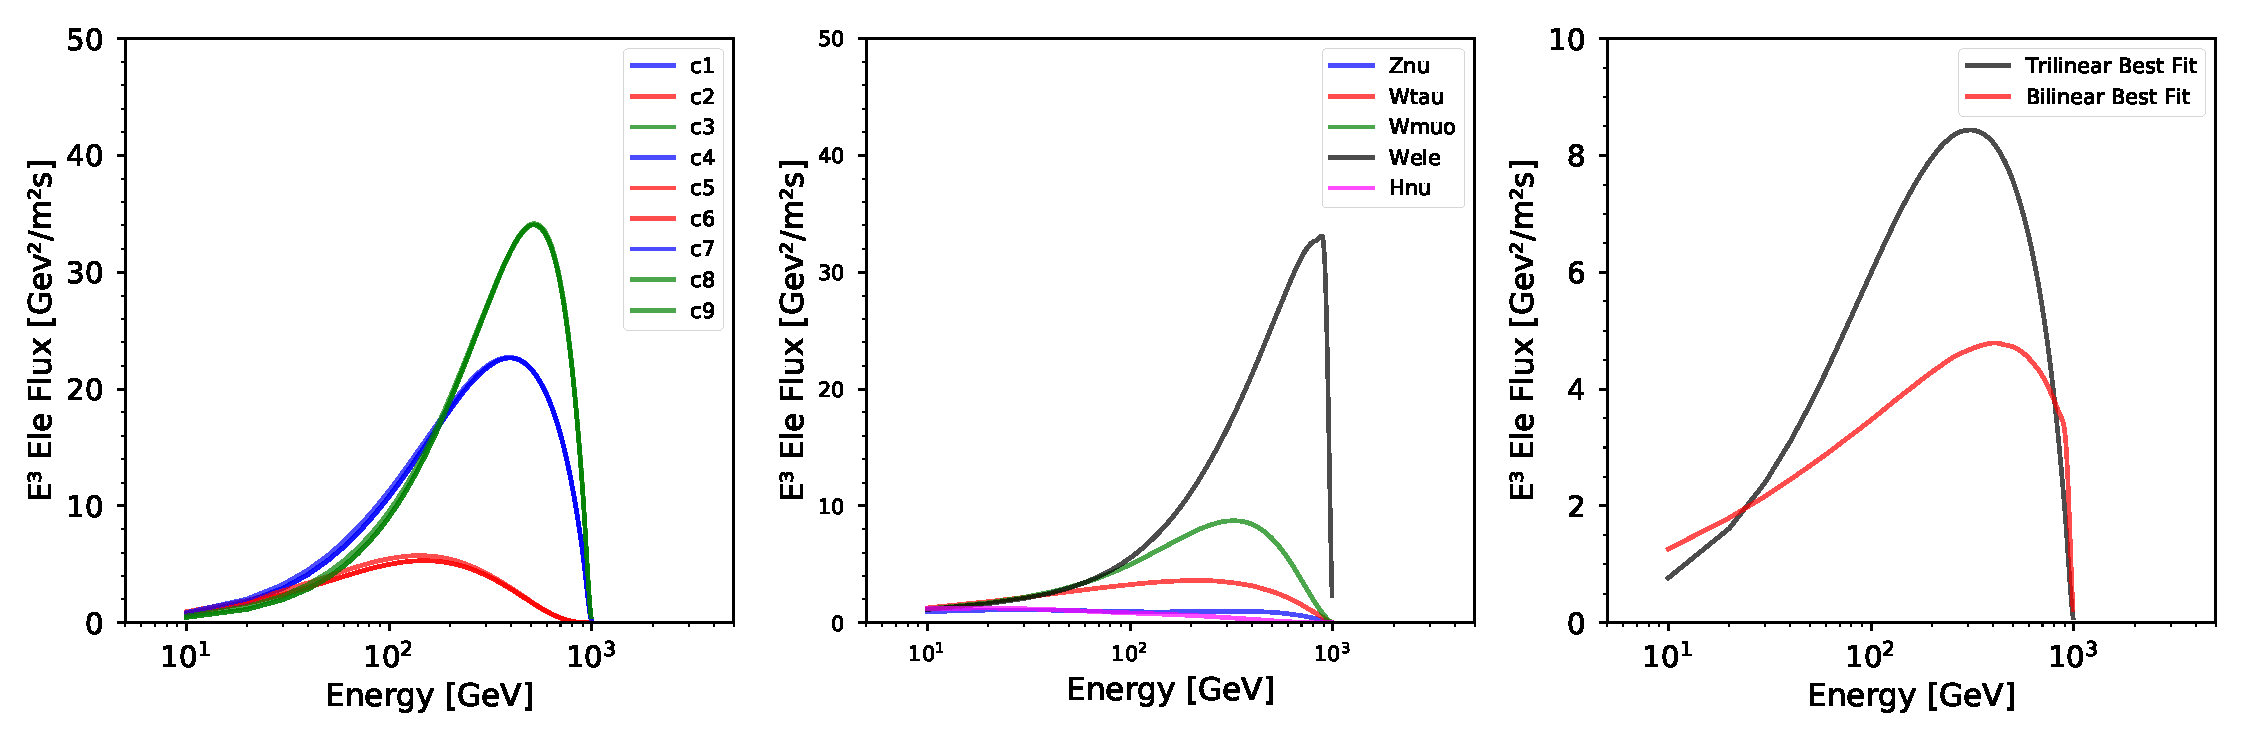
\includegraphics[height=6cm,width=16cm,angle=0]{Figures/exp_plots_electron_flux_comparison.pdf}
\caption{Charged lepton spectrum of trilinear (left) and bilinear (center) decay channels. In the right figure we show we show the contribution to charged leptons from both cases considering branching fractions that fit well the positron flux behavior.}
\label{fig:positron-spectrum}
\end{center}
\end{figure}

Furthermore, it also can be shown that for the analogous exercise but now using the photon spectrum, which is shown in Fig.~(\ref{fig:photon-spectrum}), the contribution to photons from TRpV is decreased in comparison to BRpV. Therefore, \blue{there are two contributing factors improving the performance of TRpV in comparison to BRpV}. For a given gravitino decay rate, there are both an enhancement of the charged lepton flux and a reduction of the contribution to photons that confabulate to reduce the tension with the EGB measurements.

\begin{figure}[htb]
\begin{center}
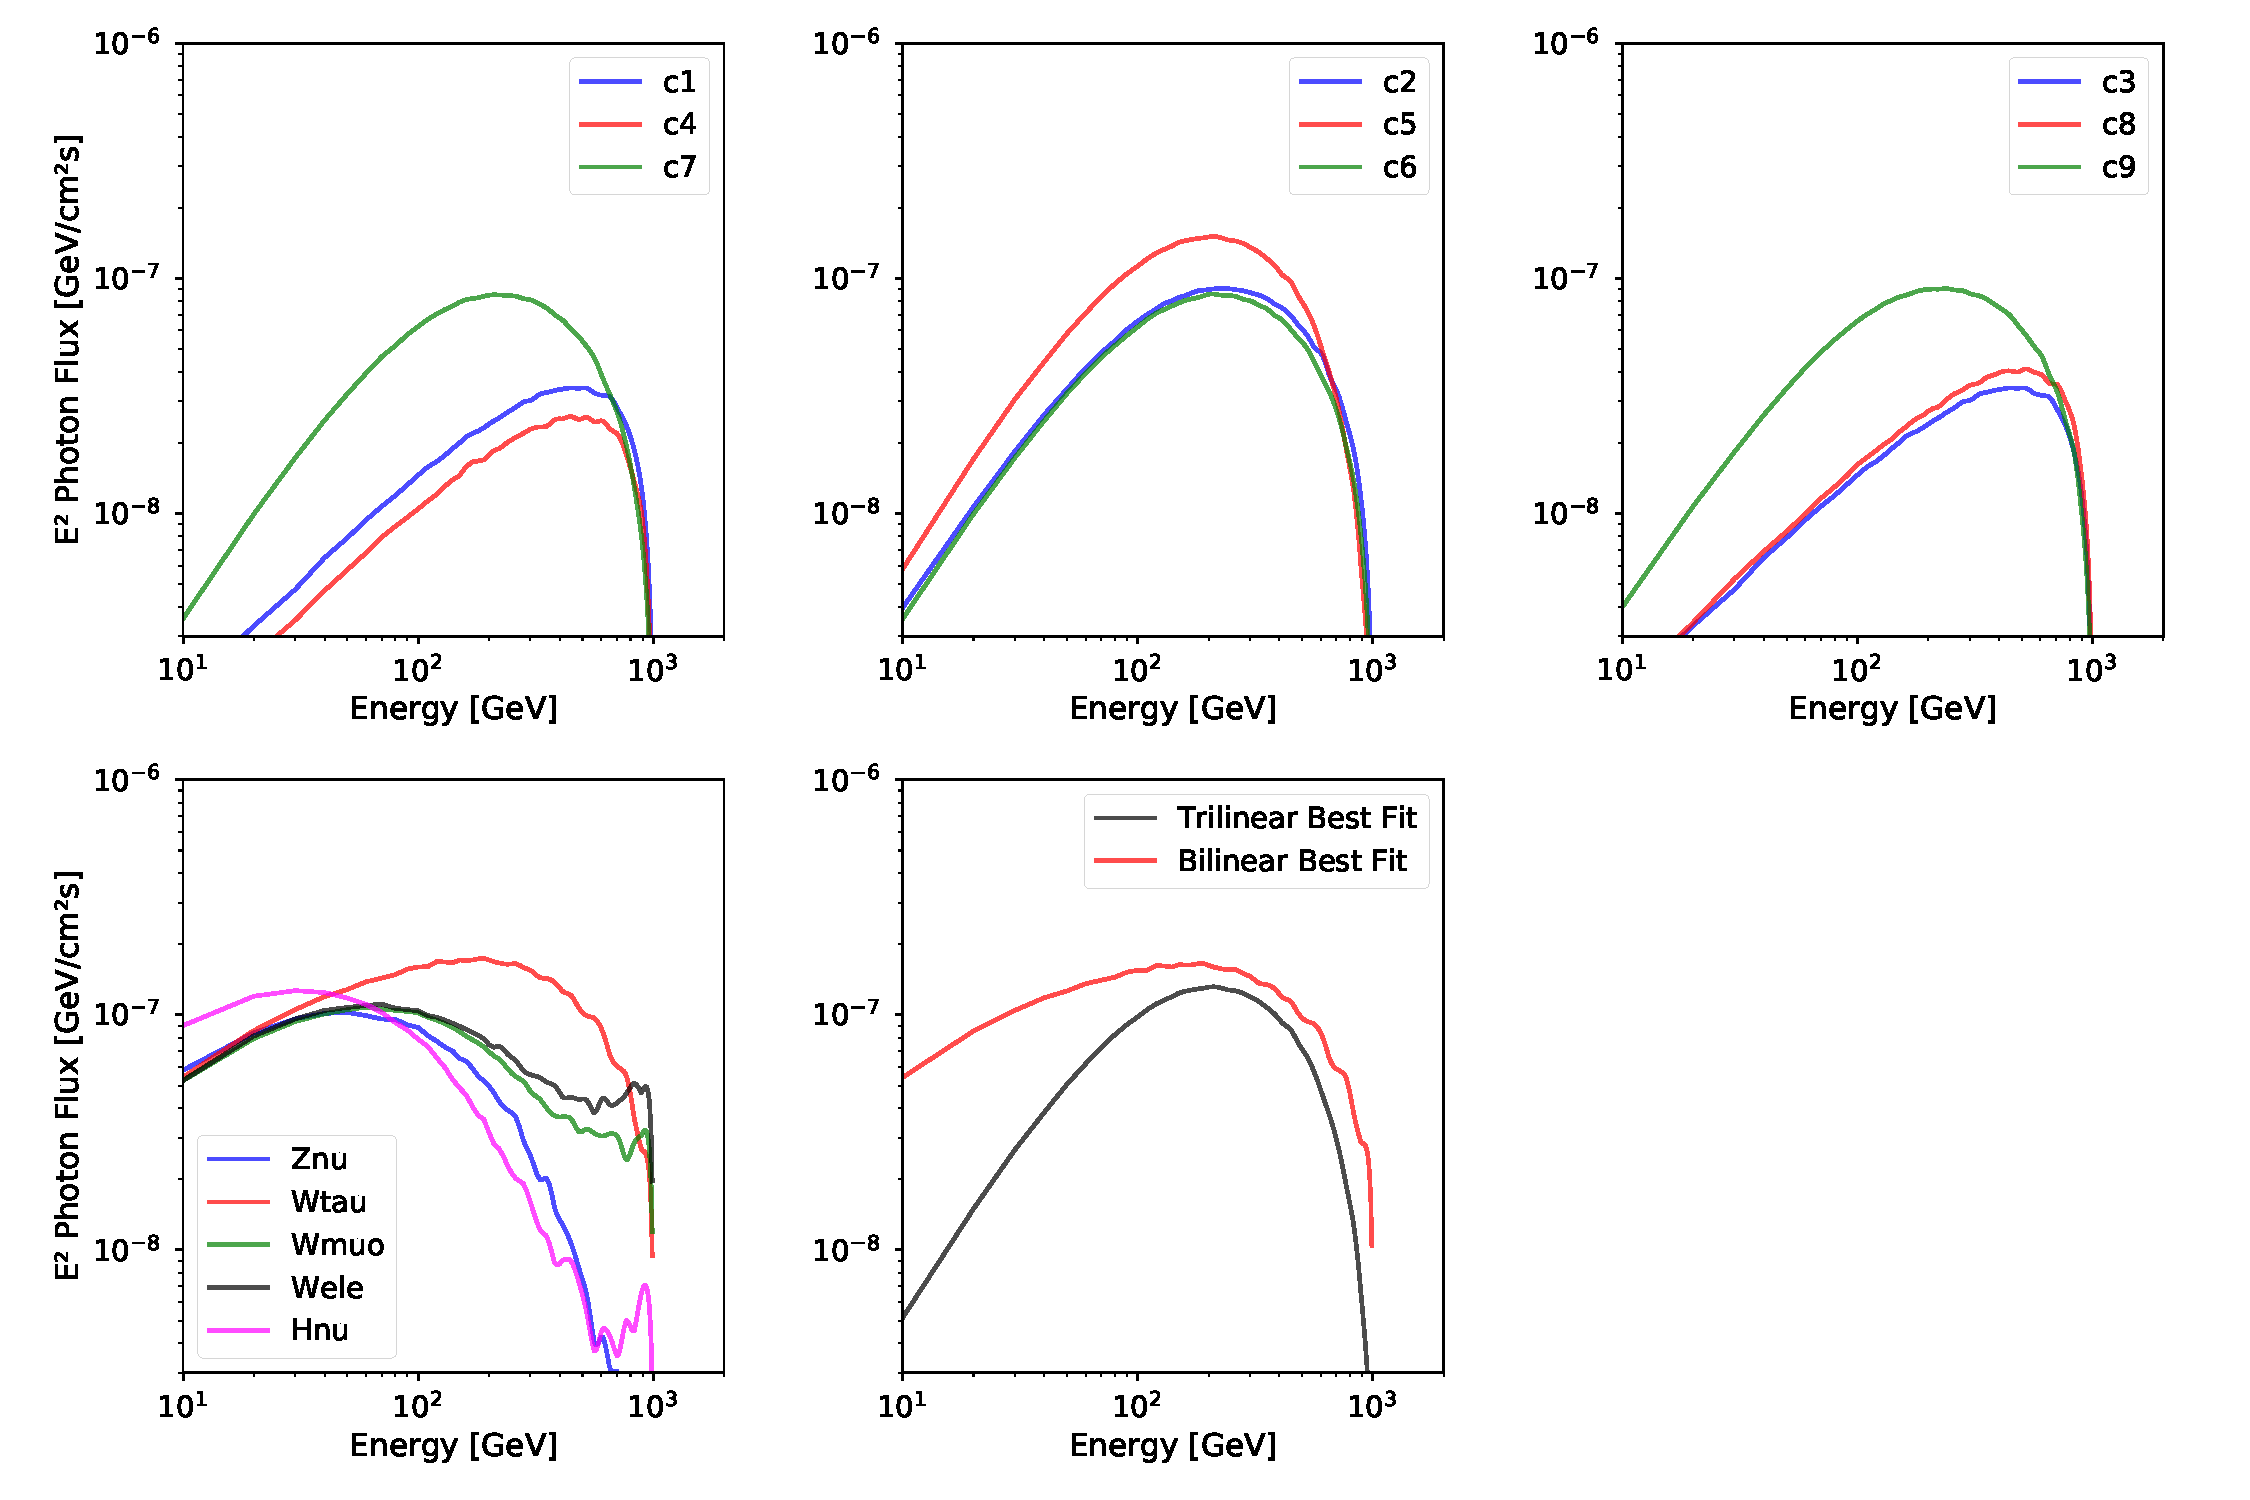
\includegraphics[height=12cm,width=16cm,angle=0]{Figures/exp_plots_gamma_rays_EGB_comparison.pdf}
\caption{Photon spectrum of trilinear (full top row) and bilinear (left bottom panel) decay channels. In the last figure (right bottom panel) we show the contribution to photons from both cases considering branching fractions that fit well the positron anomaly.}
\label{fig:photon-spectrum}
\end{center}
\end{figure}

\section{Discussion about the gravitino lifetime and neutrino masses}
\label{sec:lifetime-neutrinomasses}

The full expressions for the gravitino decay width, considering trilinear
R-Parity violation, are given in~\cite{Moreau:2001sr}. For instance, from
these expressions we can get an approximated formula for the leptonic
decay $\Gamma(\tilde{G}\rightarrow\nu_{i}e_{j}\bar{e}_{k})$ by assuming
that the mass of the sleptons that mediate the three body decay are
equal, such that $m_{\tilde{\nu}_{iL}}=m_{\tilde{e}_{jL}}=m_{\tilde{e}_{kR}}=\tilde{m}$,
and expand in taylor series around the variable $m_{G}/\tilde{m}$
to obtain

\begin{equation}
\Gamma(\tilde{G}\rightarrow\nu_{i}e_{j}\bar{e}_{k})\approx\frac{1}{96(2\pi)^{3}}\frac{\lambda_{ijk}^{2}}{8M_{\star}^{2}}\frac{m_{G}^{7}}{\tilde{m}^{4}},\label{eq:GravDecayApp}
\end{equation}


\noindent where $M_{\star}=(8\pi G_{N})^{1/2}=2.4\times10^{18}\,\mbox{GeV}$
is the reduced Planck mass. This result shows that the decay width
(lifetime) decreases (increases) rapidly as we increase $\tilde{m}$,
as expected. We expect that a similar behavior should be obtained
even when the mass of sleptons are not equal.

Indeed, we have verified this expectation numerically, by evaluating
the full expression given in~\cite{Moreau:2001sr} using the maximum numerical
precision in Mathematica. For instance, in Fig. \ref{fig:Gravitino-life-time}
we plot the gravitino lifetime as a function of $m_{\tilde{\nu}_{iL}}$
for $m_{\tilde{e}_{jL}}=m_{\tilde{\nu}_{iL}}/2$ and $m_{\tilde{e}_{kR}}=m_{\tilde{\nu}_{iL}}/5$.
Also, in the same figure we plot the lifetime derived from Eq. \ref{eq:GravDecayApp}
evaluated at $\tilde{m}=m_{\tilde{\nu}_{iL}}/2$ in order to check
that both approaches, exact computation and approximated formula,
behave similarly.

\begin{figure}
\begin{centering}
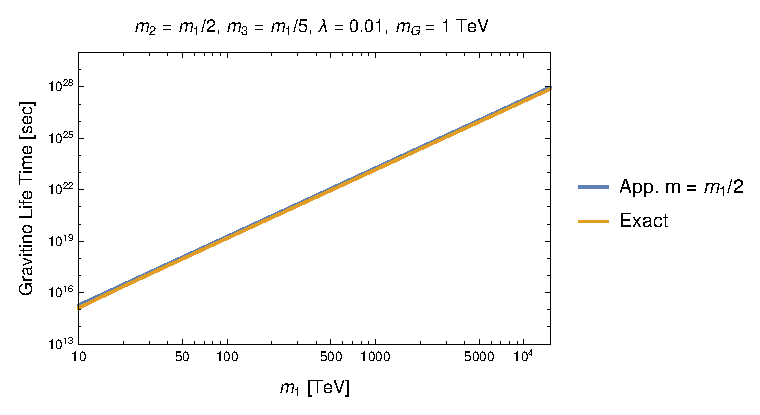
\includegraphics[scale=1.2]{GravitinoDecaym1m2m3Final}
\par\end{centering}

\caption{\label{fig:Gravitino-life-time}Gravitino life time in Trilinear RpV
for $\lambda_{ijk}=0.01,\,m_{G}=1\,\mbox{TeV}$. For simplicity we
use $m_{1},\,m_{2},\,m_{3}$ and $m$ instead of $m_{\tilde{\nu}_{iL}},\,m_{\tilde{e}_{jL}},\,m_{\tilde{e}_{kR}}$
and $\tilde{m}$.}
\end{figure}


Therefore, we can confidently derive the following expression for
the gravitino lifetime,

\begin{equation}
\tau_{G} \approx 10^{26}\,\text{s}\,\left(\frac{1}{\lambda_{ijk}\lambda_{ijk}}\right)\left(\frac{\tilde{m}}{2\times 10^{7}\mbox{\,GeV}}\right)^{4}\left(\frac{1\,\mbox{TeV}}{m_{G}}\right)^{7}\label{eq:GravLifeTime}
\end{equation}


\noindent where we have normalized with respect to $10^{26}$ s
since this is the order of magnitude required by experiments such
as AMS-02 and Fermi-LAT in order to fit the electron positron data
in the first case or to avoid gamma ray constraints in the second.


%\subsection{Neutrino Masses}

In TRpV the neutrino mass matrix receives contributions from
1-loop diagrams that contain both a charged lepton and the corresponding
slepton. Indeed, we have derived the following (preliminary) expression

\begin{eqnarray*}
M_{ij}^{\nu\,(1)} & \approx & \frac{1}{16\pi^{2}}\sum_{gr}s_{\tilde{l}}c_{\tilde{l}}(\lambda_{igr}\lambda_{jrg}+\lambda_{jgr}\lambda_{irg})m_{g}\ln\frac{m_{\tilde{l}_{r2}}^{2}}{m_{\tilde{l}_{r1}}^{2}}
\end{eqnarray*}


\noindent where $i$ and $j$ are neutrino generation indices that
runs from 1 to 3. $g$ is a charged lepton index that also run from
1 to 3, as well as $r$ which is a slepton index. Thus, it can be
seen that for order one parameters, $s_{\tilde{l}} \sim c_{\tilde{l}} \sim \ln(m_{l_{r2}}^{2}/m_{l_{r1}}^{2})\sim 1$, we can get neutrino masses around the eV scale for $\lambda_{ijk}\approx0.01$
even for $m_{g}\approx m_{e}$. 

%$s_{\tilde{l}}$, $c_{\tilde{l}}$ and $\ln(m_{l_{r2}}^{2}/m_{l_{r1}}^{2})$

Indeed, by following the expressions given in hep-ph/0410242 for the
contribution of $\lambda'$ trilinear terms, we can get by analogy
that the dominant term in the leptonic sector is 

\begin{eqnarray*}
M_{ij}^{\nu\,(1)} & \approx & \frac{1}{8\pi^{2}}\lambda_{i23}\lambda_{j32}\frac{m_{\mu}m_{\tau}A_{\tau}}{\tilde{m}^{2}}\\
 & \approx & 2\times10^{-2}\mbox{eV}\,\lambda_{i23}\lambda_{j32}\,\left(\frac{10^{8}\mbox{\,GeV}}{\tilde{m}}\right)\\
 & \approx & 2 \times10^{-2}\mbox{eV}\,(\lambda_{i23}\lambda_{j32})^{1/4}\left(\frac{\tau_{G}}{10^{\text{26}}\,\text{s}}\right)^{1/4}\left(\frac{m_{G}}{2\,\mbox{TeV}}\right)^{7/4}
\end{eqnarray*}


\noindent where $A_{\tau}$ is a free parameter that can be considered
of order $\tilde{m}$, as it is done in~\cite{Chun:2004mu}. Thus, if we
consider this formula together with Eq.~(\ref{eq:GravLifeTime}) we
see that we can have contributions to the neutrino mass matrix of
order $10^{-2}$ eV for trilinear couplings and a scalar mass
which are compatible with $\tau_{G}\approx10^{26}$ s.

\section{Conclusions}
\label{sec:conclusions}
\blue{We have presented a tri-linear gravitino decay model. Within this scenario, we can consistently} explain the data from AMS-02 and respect the EGB limits derived from Fermi-LAT data, which can be understood from the particular features of gravitino decays of this model. However, when we include the data from CALET or DAMPE, that cover higher energies than AMS-02, the things get tougher again. Nonetheles, in this model we also can connect the life-time and branching fractions of gravitino decays that are able to explain the positron anomaly to the scale of neutrino physics. 

In our computations we have not considered the extragalactic component of gravitino decays or the inverse Compton mechanism, which will enhance the contribution to the total amount of gamma-rays produced by our candidate dark matter. By considering these issues we may suggest that this scenario can accomodate most but not all of the anomalous signal in the charged lepton measurements and the rest should be supplied by astrophysicical components. 

\section*{Acknowledgments}

{\small 
\blue{We acknowledge support from the CONICYT-Chile grants Basal-CATA
PFB-06/2007 and Basal AFB-170002 (JB), FONDECYT Postdoctorados 3160439 (JB) and the Ministry of Economy, Development, and Tourism’s Millennium Science Initiative through grant IC120009, awarded to The Millennium Institute of Astrophysics, MAS (JB). BP also thanks for the support of the State of S\~{a}o Paulo Research Foundation (FAPESP).}


%The authors are thankful to Andrea Albert, Borut Bajc, Marco Cirelli, Michael Grefe, Luis Labarga, Carlos Munoz, Paolo Panci, Frank Steffen, and Gabriela Zaharijas for useful comments, and Marco Ajello for providing the EGB model contributions of Fig.~(\ref{fig:bf-photon-egb-spectrum}).
% This work was supported by Conicyt Anillo grant ACT1102. GAGV thanks for the support of the Spanish MINECO's Consolider-Ingenio 2010 Programme under grant MultiDark CSD2009-00064 also the partial support by MINECO under grant FPA2012-34694. BP also thanks for the support of the State of S\~{a}o Paulo Research Foundation (FAPESP). The work of NV was supported by CONICYT FONDECYT/POSTDOCTORADO/3140559.
}
%%%%%%%%%%%%%%%%%%%%%%%%%%%%%%%%%%%%%%%%%%%%%%%%%%%%%%%%%%%%%%%%%%

\appendix
\section{Appendix}
\subsection{Results of the fit}

In this section we show the plots concerning the statistical analysis of Cases 1 to 4, which are detailed in the main text. The black lines indicate the best fit curve, while the shade regions show 1 and 2 $\sigma$ confidence level regions.

\begin{figure}[htb]
\begin{center}
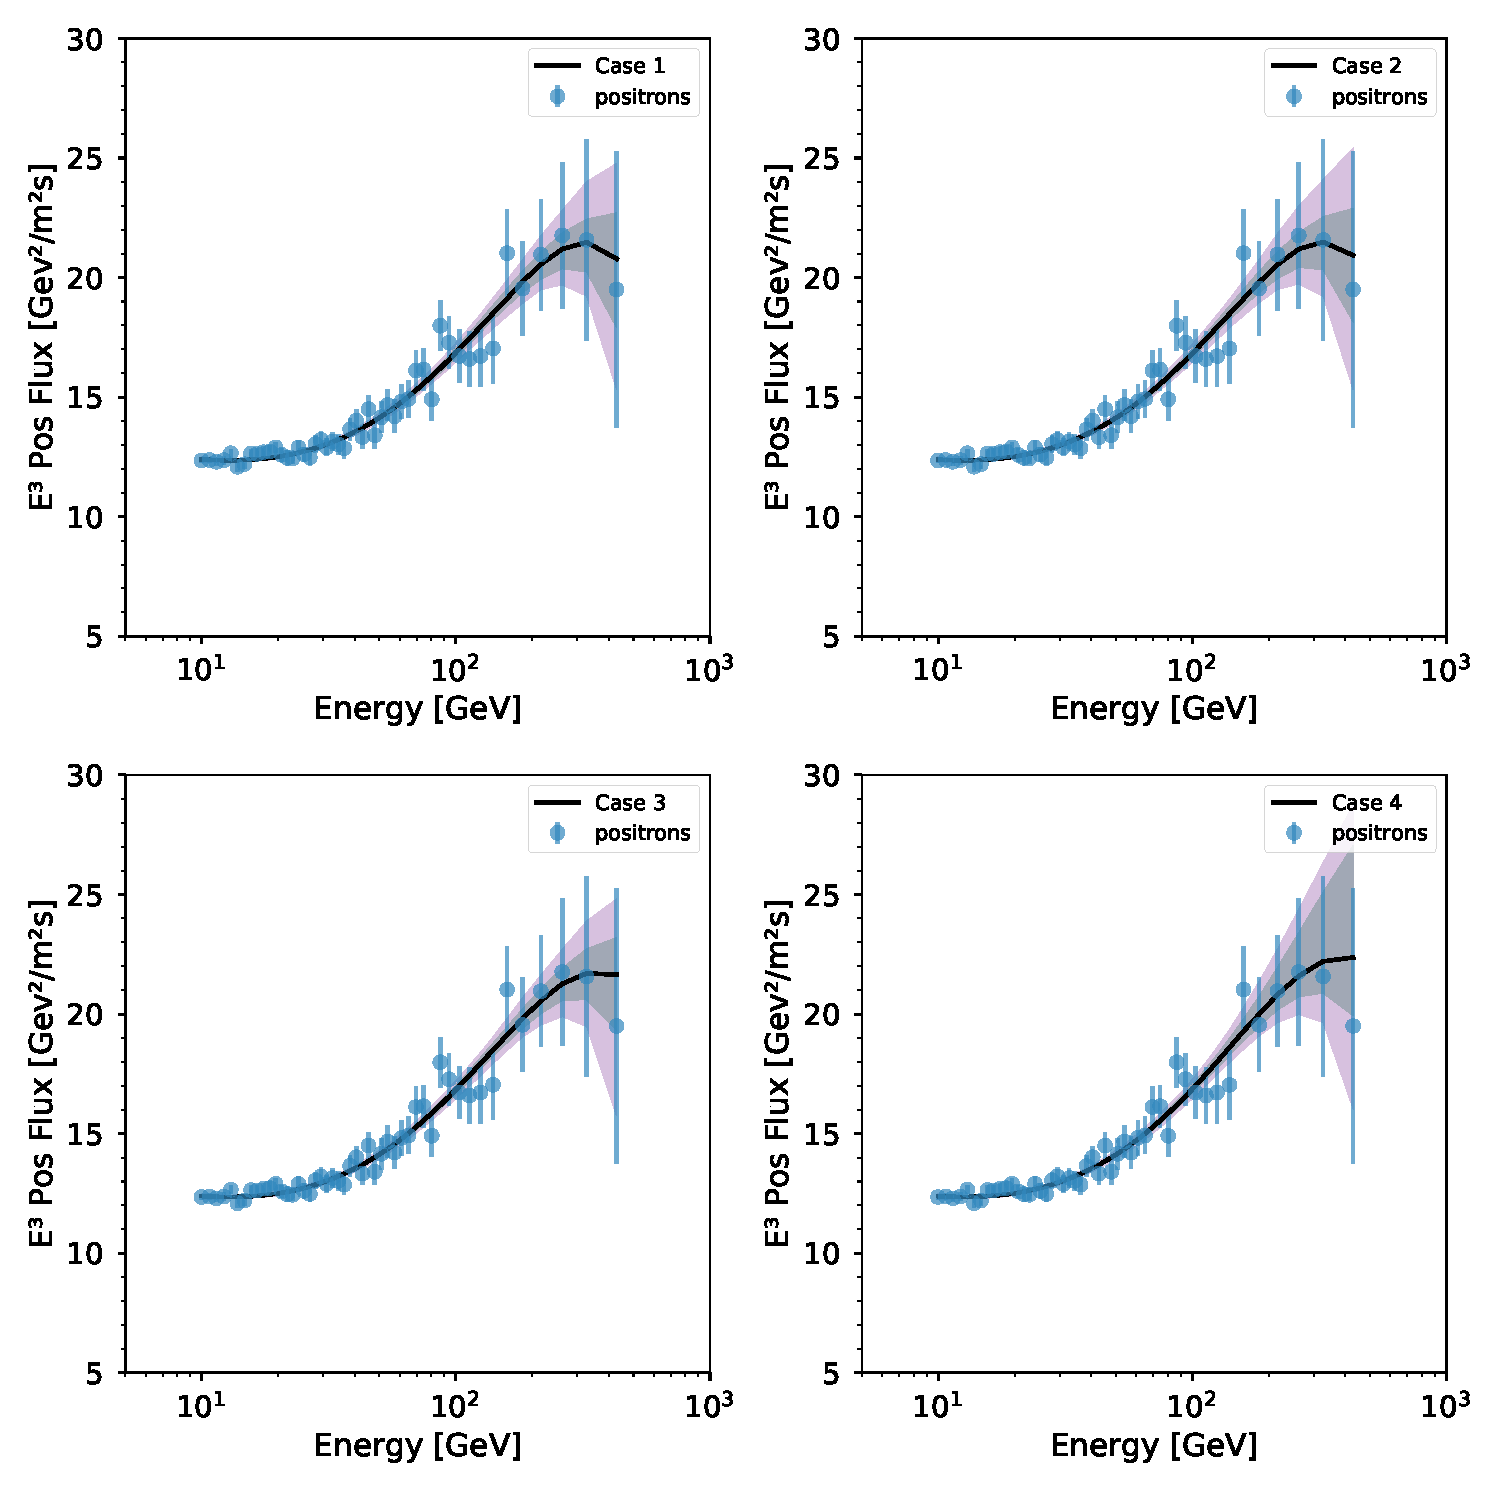
\includegraphics[height=14cm,width=14cm,angle=0]{Figures/pymultinest_fit_case_5_positron_flux.pdf}
\caption{Best fit results for positron flux. The cases $D_1$ to $D_4$ are ordered from left to right and from top to bottom.}
\label{fig:bf-positron-spectrum}
\end{center}
\end{figure}

\begin{figure}[htb]
\begin{center}
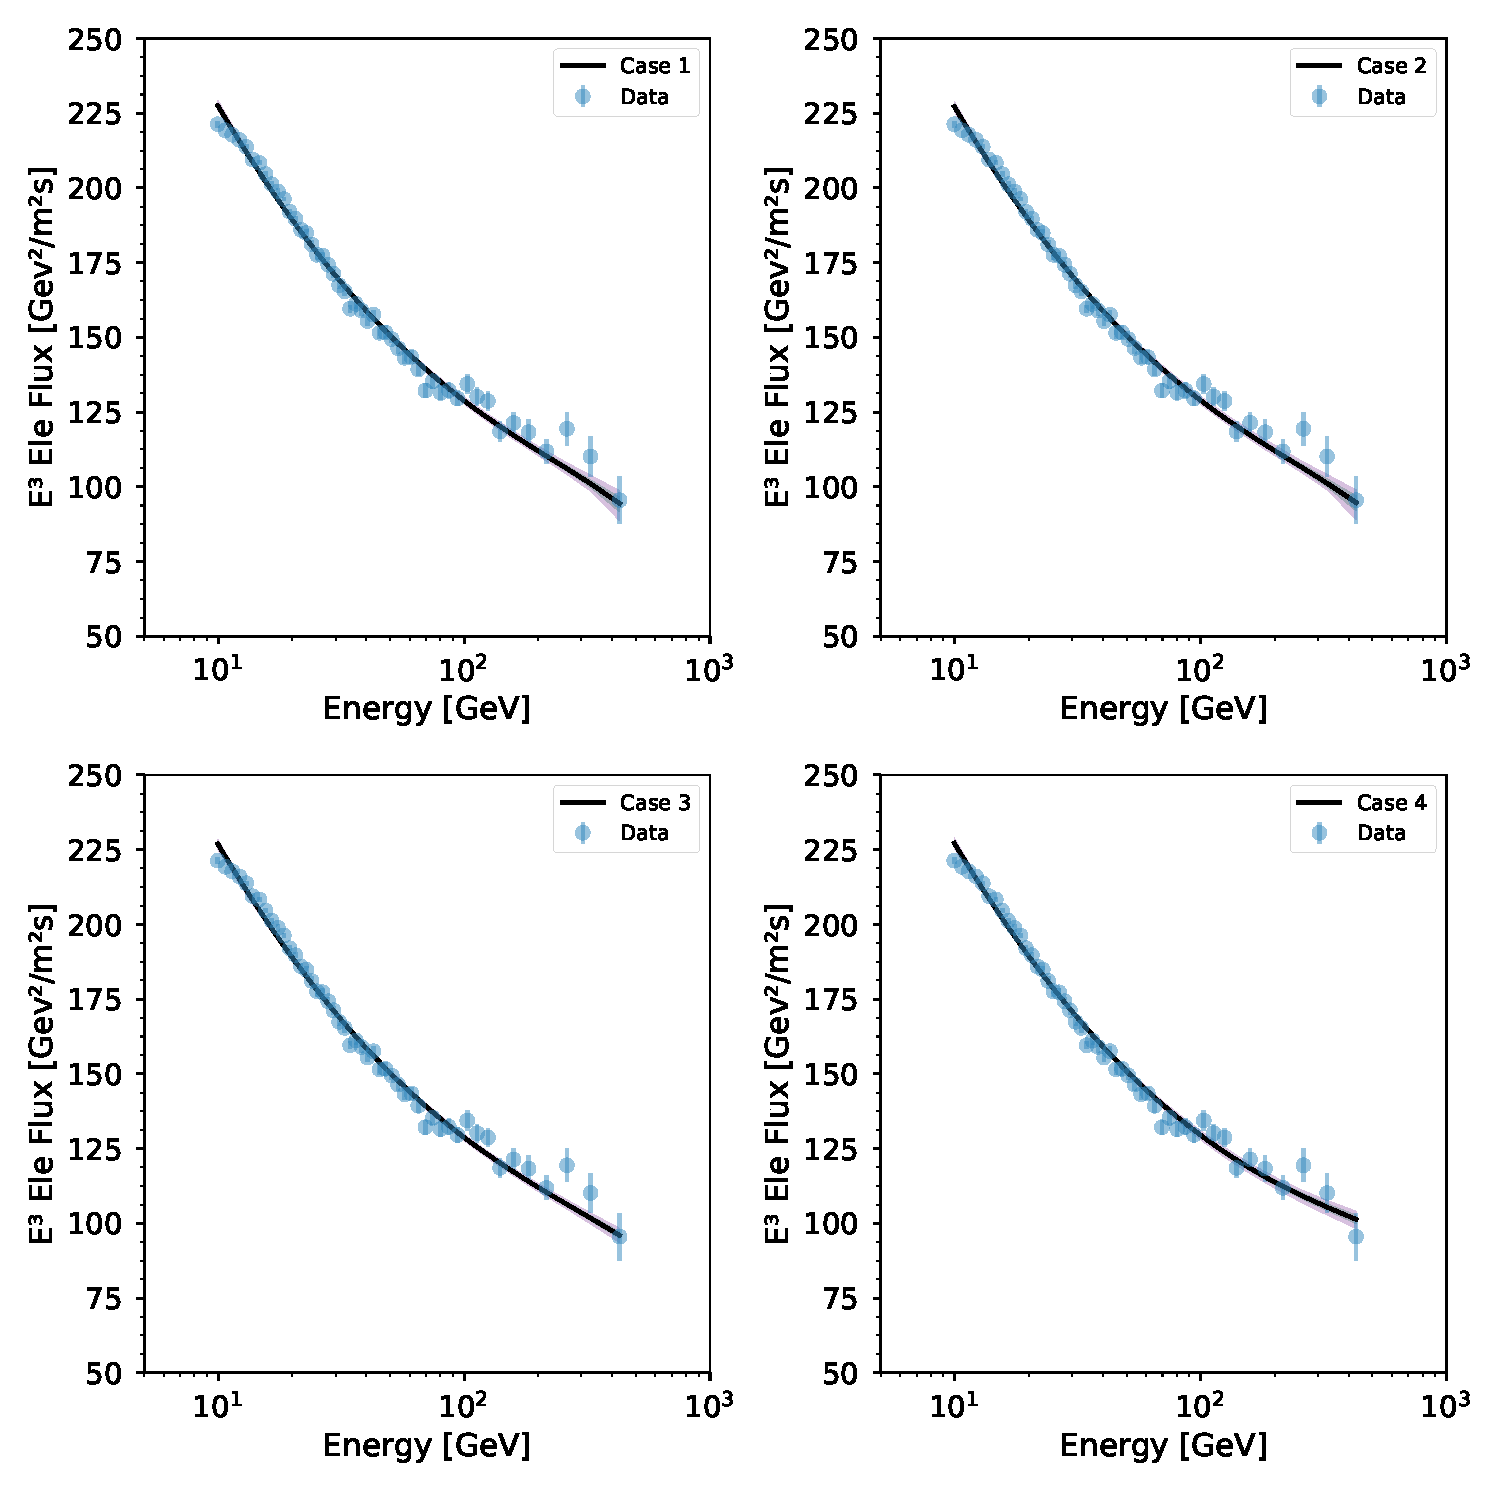
\includegraphics[height=14cm,width=14cm,angle=0]{Figures/pymultinest_fit_case_5_electron_flux.pdf}
\caption{Best fit results for electron flux. The cases $D_1$ to $D_4$ are ordered from left to right and from top to bottom.}
\label{fig:bf-electron-spectrum}
\end{center}
\end{figure}

\begin{figure}[htb]
\begin{center}
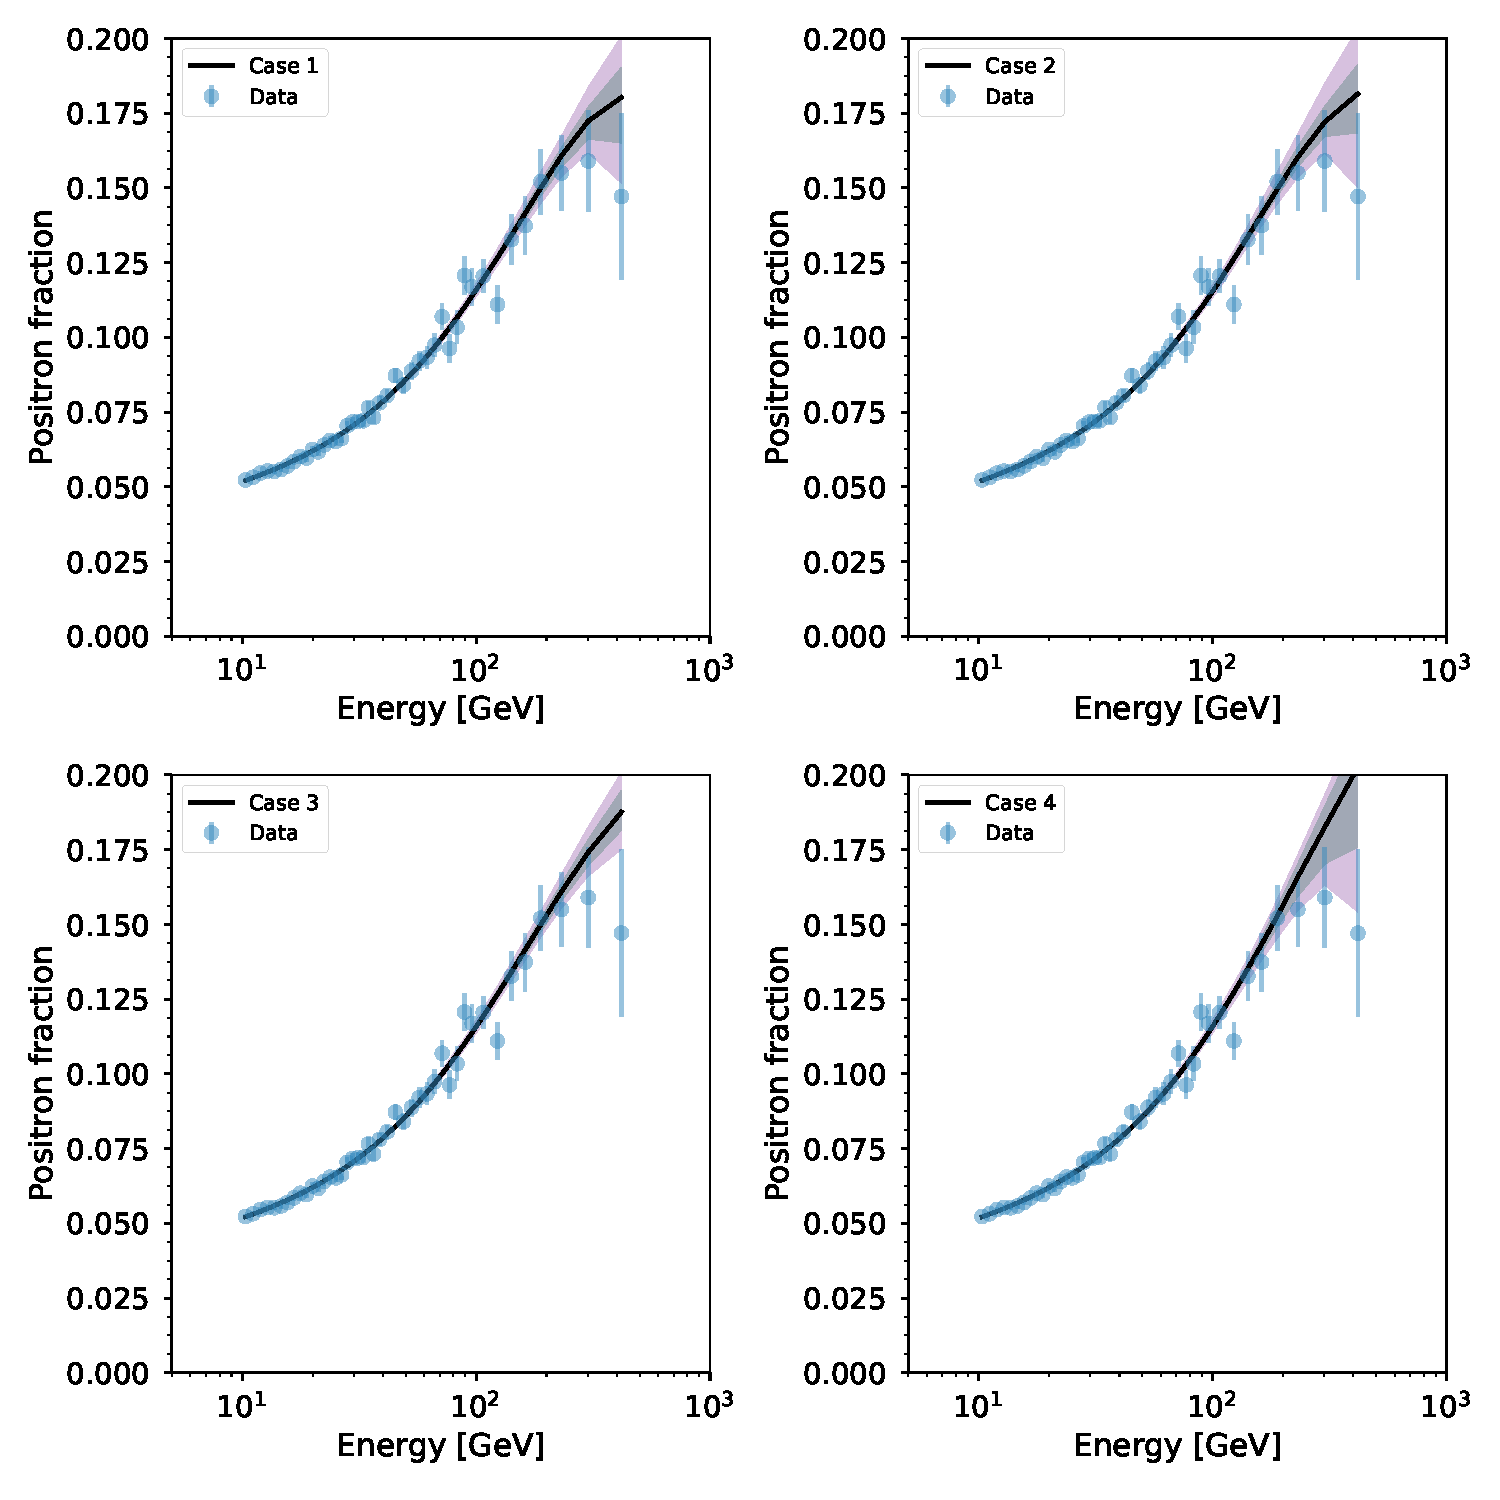
\includegraphics[height=14cm,width=14cm,angle=0]{Figures/pymultinest_fit_case_5_ep_fraction.pdf}
\caption{Best fit results for positron fraction. The cases $D_1$ to $D_4$ are ordered from left to right and from top to bottom.}
\label{fig:bf-positron-fraction-spectrum}
\end{center}
\end{figure}

\begin{figure}[htb]
\begin{center}
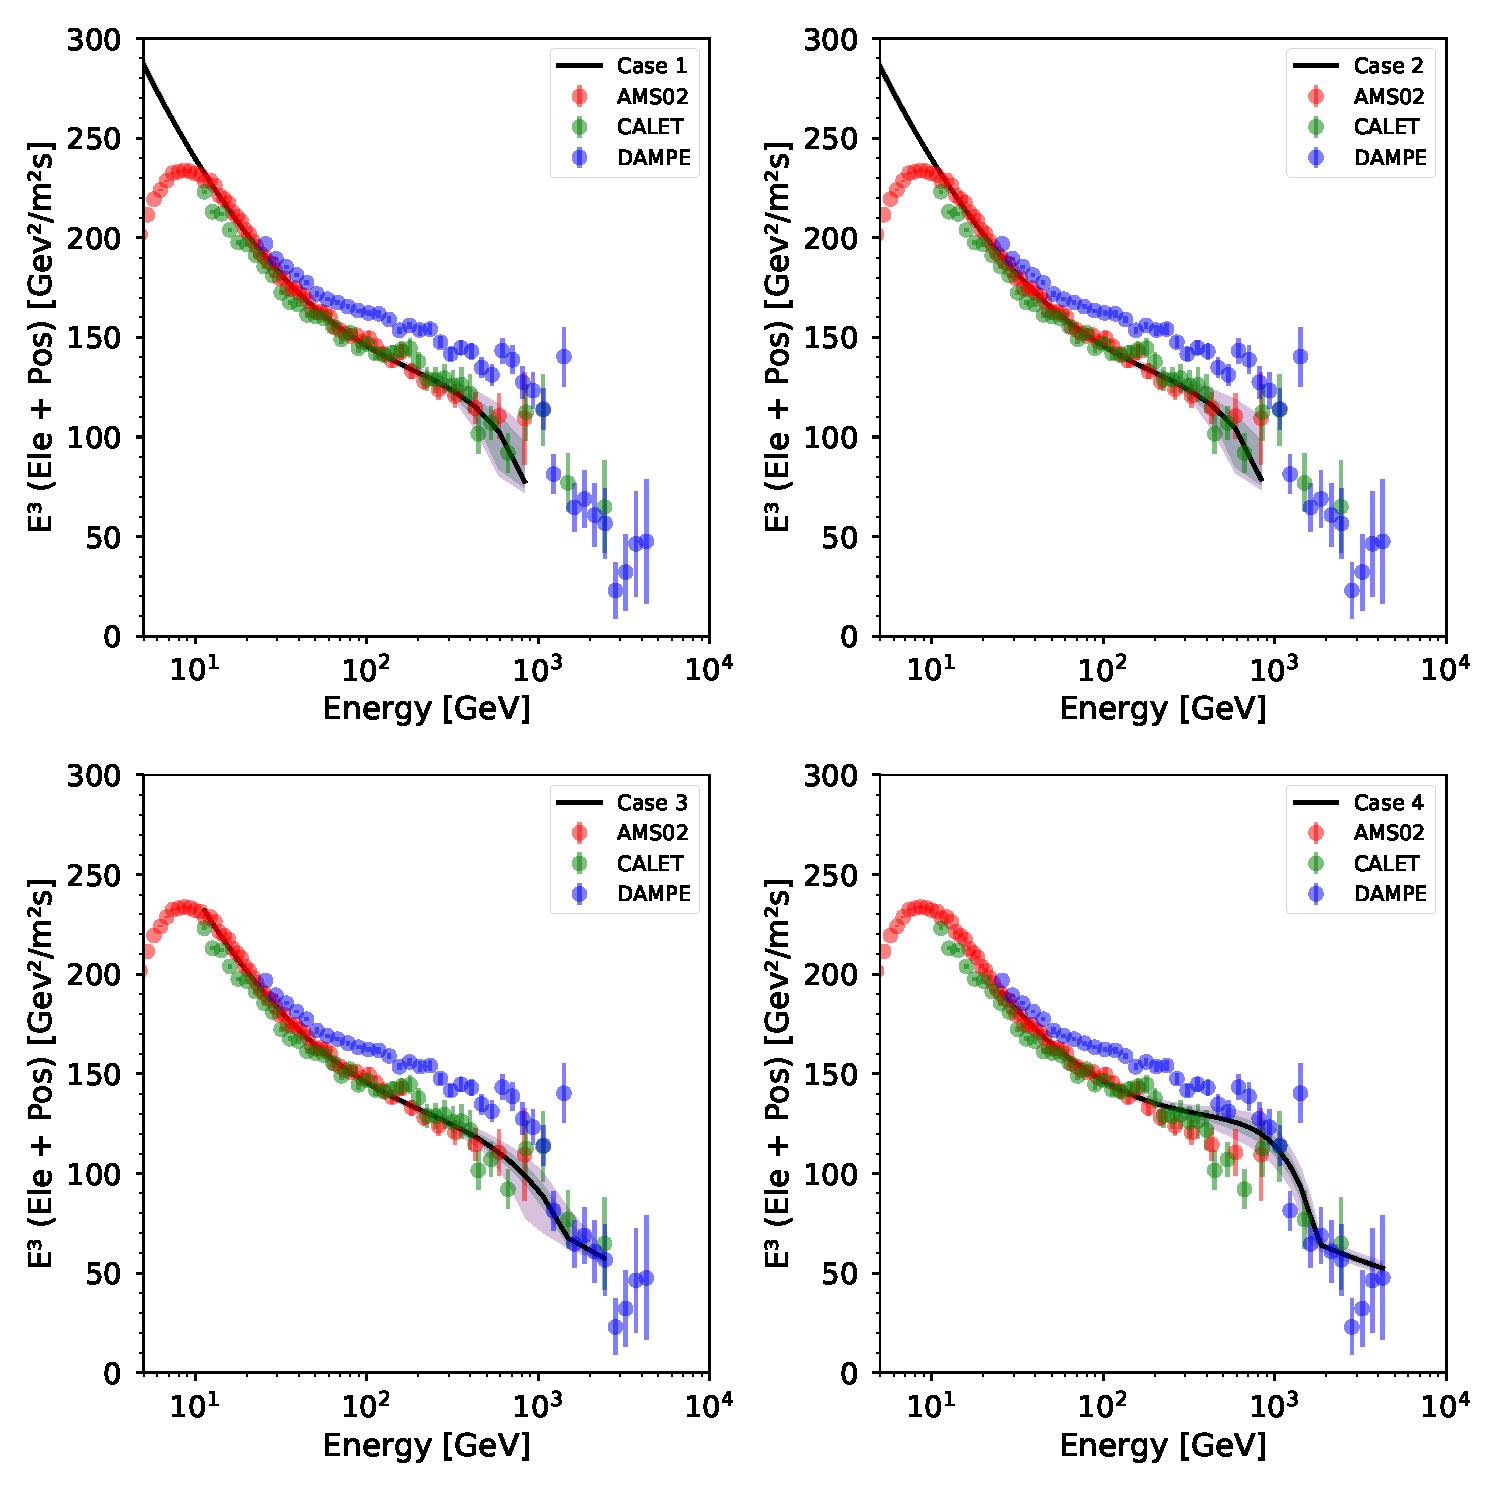
\includegraphics[height=14cm,width=14cm,angle=0]{Figures/pymultinest_fit_case_5_electron_plus_positron.pdf}
\caption{Best fit results for electron plu positron flux. The cases $D_1$ to $D_4$ are ordered from left to right and from top to bottom.}
\label{fig:bf-electron-plus-positron-fraction-spectrum}
\end{center}
\end{figure}

\begin{figure}[htb]
\begin{center}
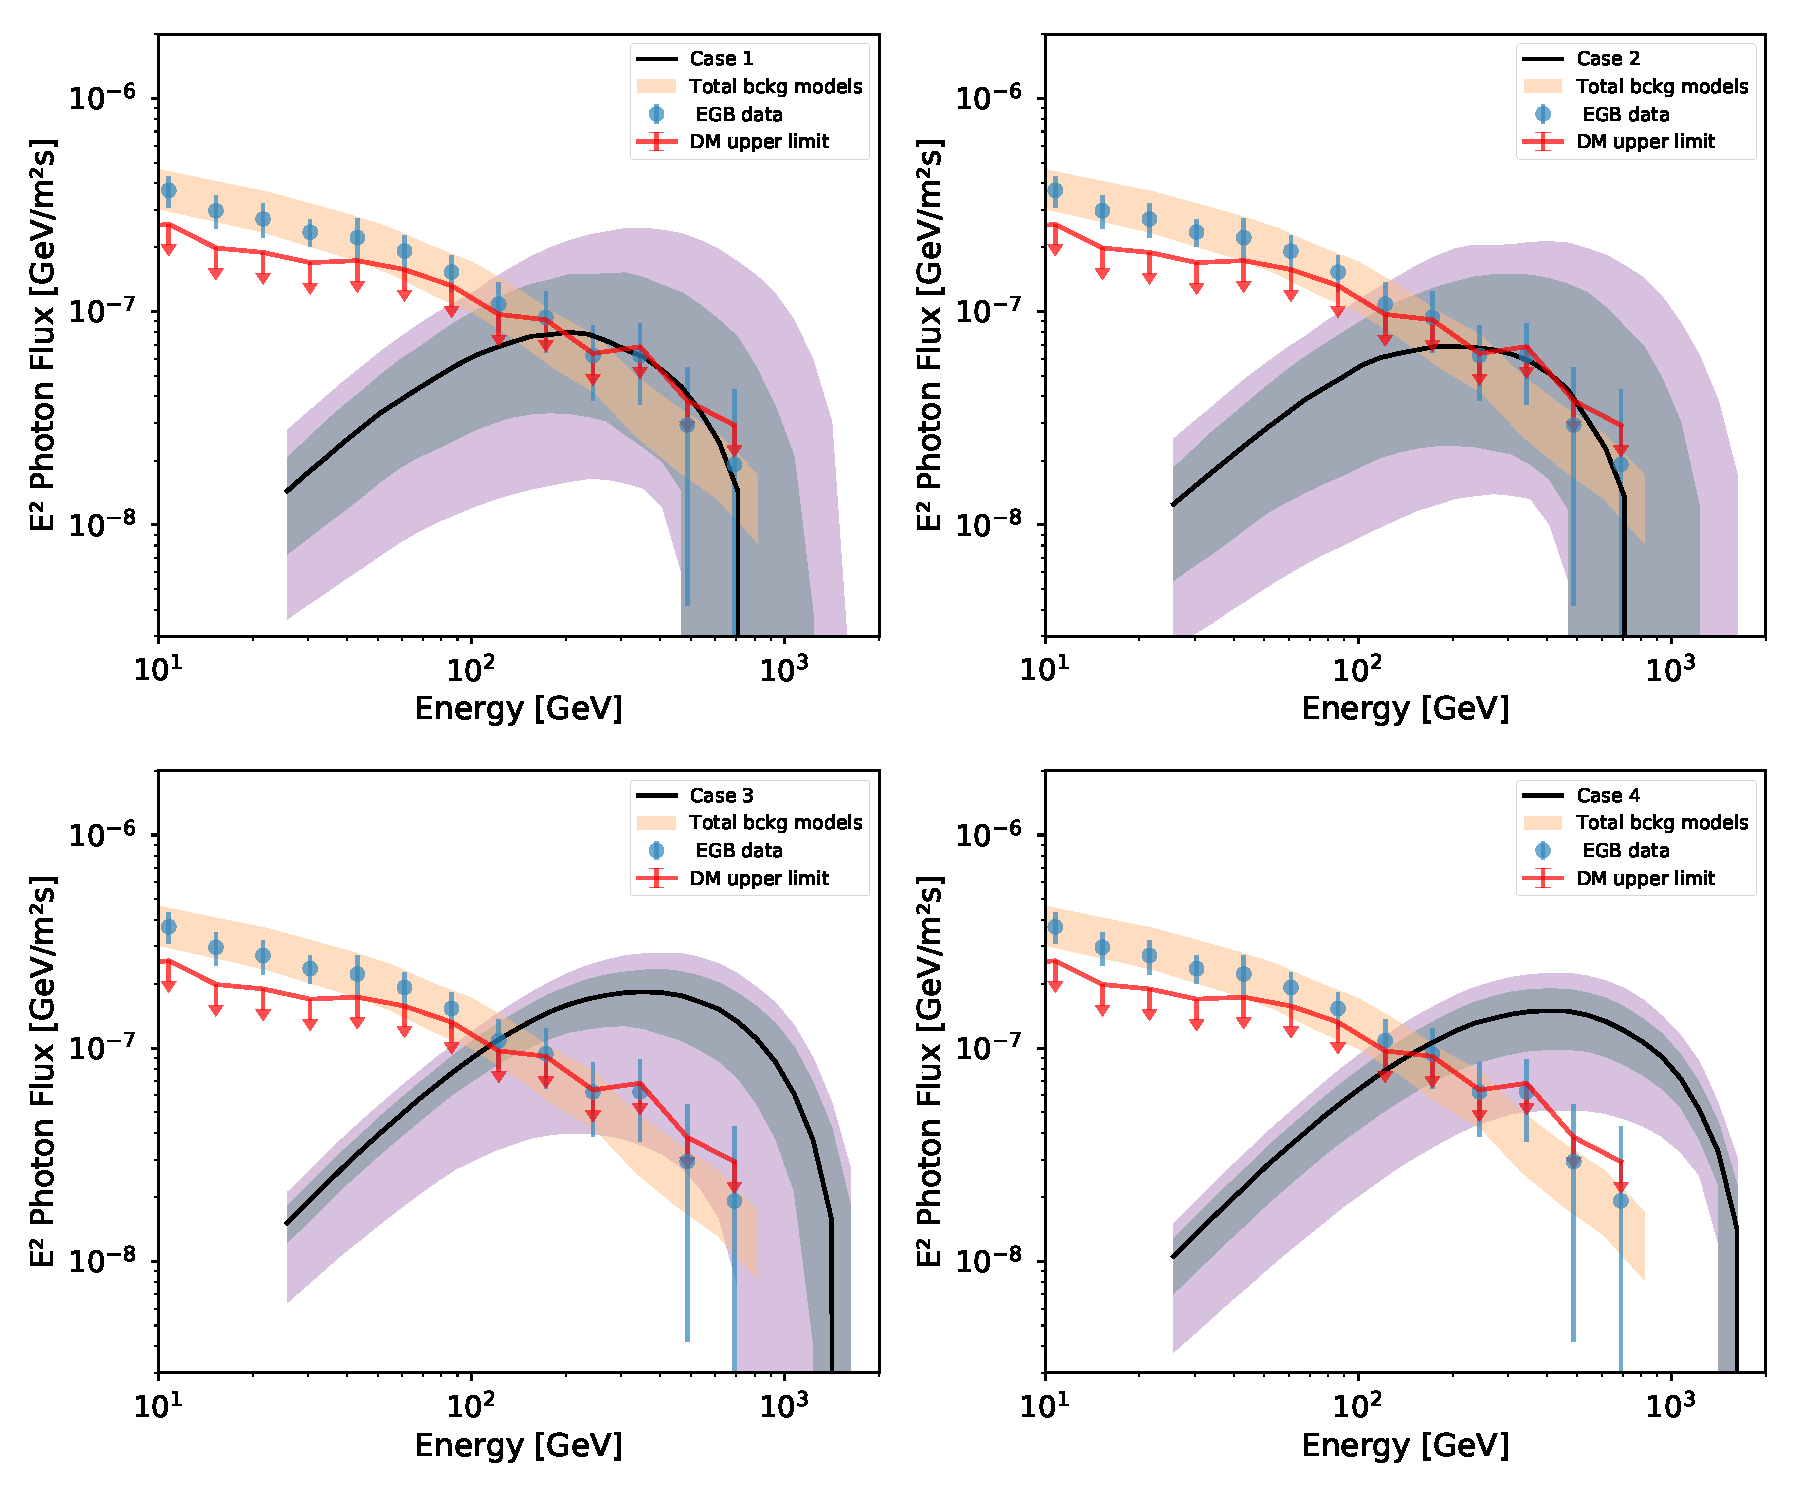
\includegraphics[height=12cm,width=16cm,angle=0]{Figures/pymultinest_fit_case_5_gamma_rays_EGB.pdf}
\caption{Best fit results for photon fluc compared to EGB limits. The cases $D_1$ to $D_4$ are ordered from left to right and from top to bottom.}
\label{fig:bf-photon-egb-spectrum}
\end{center}
\end{figure}

%\newpage
\clearpage
\bibliographystyle{JHEP}
\bibliography{Gravitino_Trilinear_References}

\end{document}


